\documentclass[12pt]{article}
\usepackage{dirtree}
%\usepackage{cite}
\usepackage[utf8]{inputenc}
\usepackage{listings}
\usepackage{pdfpages}
\usepackage{fancyhdr}
\usepackage{biblatex}
\addbibresource{bibilo.bib}
\usepackage{tocloft}
%\renewcommand{\cftsecleader}{\cftdotfill{\cftdotsep}}
%\renewcommand{\cftsecpagefont}{}% Remove \bfseries from section titles' page in ToC
\usepackage{verbatim}
\usepackage{amsmath}
\usepackage[utf8]{inputenc}
%\newcommand\logoPath{TU-logo.png}
%\newcommand\logoFileName{TU-logo}
%\newcommand\logoScaleFactor{0.7}
\usepackage{graphicx}
\usepackage{setspace}
\usepackage{afterpage}
\usepackage{tikz}
\usetikzlibrary{shapes,arrows, positioning}
\usepackage{abstract}
\renewcommand{\abstractnamefont}{\normalfont\large\bfseries}
\begin{document}
\graphicspath{\logoPath}
\renewcommand*\contentsname{Table Of Contents}
\newcommand\myemptypage{
		\null
		\thispagestyle{empty}
		\addtocounter{page}{-1}
		\newpage
}
\lstdefinestyle{mystyle}{frame=tb,
						%language=C++,
						tabsize=3,
						numbersep=5pt}
\lstset{style=mystyle}
\begin{titlepage}
  \begin{center}
      \textbf{
      	  \begin{huge}Project Proposal:\\ \end{huge}
      	  \begin{huge}
      	  geocold\\
			Ray Tracer (Differentiable?) in C++
			\end{huge}}\\
    \vspace{0.5\baselineskip}
    {\Large Authors:  Prakash Chaulagain, Nishar Arjyal, and Pramish Paudel}\\
   	\Large{Roll Numbers: 076BCT045, 076BCT042, 076BCT047} \\
   	\vspace{0.5\baselineskip}
    \centering
      Submitted to the Department of
      Electronics and Computer Engineering
      in Partial Fulfillment of the Requirements of the 3rd Year \textbf{Computer Graphics} Course  
    at 	\\
    {\Large Pulchowk Campus }\\
    {\Large IOE, Tribhuwan University}\\
    \vspace{0.3\baselineskip}
    \today\\
  \end{center}
  \vspace{2\baselineskip}
  {
  \raggedright
		Accepted by: \dotfill

  \raggedleft
  \vspace{1\baselineskip}
  Mr. Basanta Joshi\\
  Assistant Professor at \\
  The Department of Electronics and Computer Engineering\\
  }
  \vspace{2\baselineskip}	
	 Date of Submission: \today \\
  	Expected Date of Completion: August, 2022 
\end{titlepage}
\myemptypage
\begin{center}
	{\large \textbf{Mathematical Toolkit}}\\
	by
	{Prakash Chaulagain, Nishar Arjyal, and Pramish Paudel}\\
	\vspace{0.2\baselineskip}
	\begin{spacing}{0.8}
	{Submitted to the Department of Electronics and Computer Engineering \\
	on \today \\ in Partial Fulfillment of the Requirements for the 3rd Year 
	Computer Graphics Course in Computer Engineering}\\
	\end{spacing}
\end{center}
\begin{abstract}
Derivatives and matrices seem to be ubiquitous in all of mathematical 
optimization and machine learning nowadays. In such times, it becomes
all the more important that the average computer programmer has access
to a software package that is powerful yet simple to learn in order to 
do fast gradient computations alongside a linear algebra package that-
while-using feels native to the programming language of choice. The purpose
of this project is to come up with one such mathematical package to 
fulfil the requirements of academics for either soft-core academic work 
or small-scale projects that require some form of mathematical optimization
in C++. With MathematicalToolkit we aim to give the user a native C++ 
experience in calculating derivatives of their functions.\\
Several different methods exist for calculating the derivatives of 
functions. Numerical and Symbolic are the first that come to mind. However, 
when it comes to computer programming, the programming world seems to 
have unanimously decided that the best method for a computer to differentiate
functions is by using a set of techniques called Automatic Differentiation
(see \cite{griewank} ).
Automatic Differentiation (AD) is simply the most efficient family of 
techniques for accurately calculating the derivatives of 
functions. Several techniques exist in AD (see \cite{baydin2018automatic}), 
however, the goal of this project is to implement only the Forward-Mode Automatic Differentiation
using the operator overloading approach. This project also aims 
to build a wrapper linear algebra sub-package for simple yet efficient 
matrix and vector related computations.

\end{abstract}

\newpage


\tableofcontents
\newpage

\begin{section}{Acknowledgement}
	Our project idea is the product of excellent supervision of all of our 
	instructors, most notably our lecturer Mr. Basanta Joshi. We could not 
	have been able to develop interest in computer graphics as a field of study 
	without the constant inspiration provided to us by all of our lecturers and 
	lab instructors and assistants. Some of the credit should also go to 
	the college administration for their efforts in the smooth functioning 
	of all of our classes and labs safely and securely despite the unprecedented 
	times of the pandemic. 
\end{section}

\newpage

\newpage
\pagestyle{fancy}
\fancyhead[C]{MATHEMATICALTOOLKIT}
\fancyhead[L]{}
\renewcommand{\headrulewidth}{0pt}
\renewcommand{\footrulewidth}{0pt}
\section{Objectives}
\begin{itemize}
	\item To bring Automatic Differentiation in a mathematical library
			that is suitable to use for academics.
	\item To analyze Object Oriented Programming design. 
	\item To get familiar with program optimization and safe memory-handling
	practices.
\end{itemize}
\section{Introduction}
The most popularly used method for the computation of derivatives of 
functions or mathematical expressions in computer program form when
it comes to mathematical optimization problems or machine learning 
is \emph{automatic differentiation}, also called 
\emph{algorithmic differentiation} which is the major subject 
matter of this project. 

Conventionally, most of the algorithms of optimization have 
relied heavily on computing derivatives and gradients of functions
(see \cite{kochenderfer}\footnote{\label{kochenderfer}https://mitpress.mit.edu/books/algorithms-optimization}).
Multiple implementations of automatic differentiation exist in 
various programming languages such as in C++ (Carpenter et al., 2015 \cite{carpenter2015stan})
as well as some higher level programming languages like Julia (see \cite{RevelsLubinPapamarkou2016})
However, most of these implementations are built to be used specifically
in machine learning and not for academic work. Furthermore, most 
such implementations are the reverse mode automatic 
differentiation which is more suitable in machine learning but 
perhaps less suitable in mathematics as we normally use. We aim to 
provide a very naive and incredibly hackable AD package that is 
usable for the clueless as much as it is for the pros. 


%\subsection{Finite Differencing:}
%Before talking about our implementation of automatic differentiation
%, we would like to express that MathematicalToolkit also aims to 
%provide to the user the facility of numeric differencing.
%The Taylor's expansion of a function $f(x)$ about a point $a$ $(x-a=h)$ as a funciton 
%of $x$ is: 
%$$
%f(x) = \sum_{n=0}^{\infty}\cfrac{f^{(n)}(a)}{n!}(x-a)^{(n)}
%$$
%This gives us a forward difference of a function at $a$ using only the 
%first order terms with small difference as:
%\begin{equation}
%f'(a) \approx \cfrac{f(a+h)-f(a)}{h} 
%\end{equation}
%In case of a function with multiple variables, our library intends the user 
%the following facility:
%
%If $f(\textbf{x})$ is a function of multiple variables $\textbf{x}$ where
%$\textbf{x}$ is of length n, the gradient of such a function is 
%evaluated at point $\textbf{a}$ by calculating the directional 
%derivatives in the concerned direction and storing the results in 
%a vector in the stack.
%Here, \textbf{a} has the same size as \textbf{x}.
%\begin{equation}
%	\nabla f(\textbf{a}) = \left[ \cfrac{\partial f(\textbf{a})}{\partial x_{i}}\right] for~i = 0:n-1
%\end{equation}

\subsection{Scalar Dual Numbers and Forward Mode AD}
The \emph{scalar dual number} type implemented in our library is defined as: 
\begin{equation}
	\boxed{
		f(x + y\epsilon) = f(x) + yf'(x)\epsilon + \mathcal{O}(\epsilon^{2})
}
	\label{scalardualdefine}
\end{equation}
The definition of the scalar dual number in equation~\ref{scalardualdefine}
contains a primal/value part '$x$' and a derivative part '$y$'.
Following eqn.~\ref{scalardualdefine}, we obtain 
the derivative of any function through eqn.~\ref{dualdiff}
\begin{equation}
	\boxed{
	f'(x) = \cfrac{f(x+y\epsilon) - f(x)}{y\epsilon}
}
	\label{dualdiff}
\end{equation}
By defining some dual number arithmetic through operator overloading 
such as: 
\begin{equation}
	\boxed{
	(x_{1}+y_{1}\epsilon) + (x_{2}+y_{2}\epsilon) = (x_{1}+x_{2}) + (y_{1}+y_{2})\epsilon
}
	\label{dualadd}
\end{equation}
We can achieve this easily by overloading the '+' operator over 
our custom scalar '\emph{Dual}' type. 
\\

The eqn.\ref{dualmult} is the definition of the product of two dual types.
\begin{equation}
	\boxed{
	(x_{1}+y_{1}\epsilon) \times (x_{2}+y_{2}\epsilon) = (x_{1}x_{2}) + (x_{1}y_{2}+x_{2}y_{1})\epsilon
}
	\label{dualmult}
\end{equation}
So, basically we are defining the basic derivative formulae on the 
dual type, and for chained functions, we define a set of chain rules. 
In this way, we can obtain the derivative of all scalar functions that depend
on only one variable.
\\
The $\epsilon$ in all of these formulae is called the $machine-epsilon$
defined as: $\epsilon^{2} = 0$ in the computer.
The epsilon is defined as such: 
1.0 + $\epsilon$ == 1.0 returns a true in the computer program.
So, basically, when we add or subtract a number from or to an $\epsilon$
we have done literally no computation. Further, all higher powers of 
$\epsilon$ are zero.
\subsection{Multidimensional Dual Numbers and Vector Forward Mode AD}
The scalar type mentioned above works suitably for scalar one-variable 
functions; however, better approach can be taken in the case of 
multivariate functions.
\\
Let's analyze how we can differentiate a function of two variables 
using our scalar dual numbers.
The $L_{2}$ norm of a vector $\overrightarrow{x}$ of length $n$ is defined to 
be (the indices are chosen to be the same as those used in programming 
normally).

\begin{equation}
	\boxed{
	||\overrightarrow{x}|| = \left(\sum_{i=0}^{i=n-1}x_{i}^{2}\right)^{\cfrac{1}{2}}
}
	\label{l2norm}
\end{equation}
Let us try finding the gradient of the square of this functions when the input 
has two elements.
\begin{equation}
	\boxed{
f(x_{0},x_{1}) = x_{0}^{2} + x_{1}^{2}
}
\end{equation}
First, the partial derivative with respect to $x_{0}$ is found 
by noticing that the derivative of $x_{0}$ w.r.t. $x_{0}$ itself is 
1 and the  derivative of $x_{1}$ w.r.t. $x_{0}$ is 0. \\
So basically, we are passing the dual number into the function which 
returns the value alongside the derivative as a dual number.
\begin{align}
	f(x_{0}+\epsilon, x_{1}) &= (x_{0}+\epsilon)^{2} + x_{1}^{2}  \\
	f(x_{0}+\epsilon, x_{1}) &= x_{0}^{2} + 2x_{0}\epsilon + \epsilon^{2} + x_{1}^{2} \\
	f(x_{0}+\epsilon, x_{1}) &= (x_{0}^{2}+x_{1}^{2})+ 2x_{0}\epsilon  
\end{align}
Notice from the second equation above to the third, we used the definition 
that $\epsilon^{2}$ is 0 and so are all higher powers of $\epsilon$
\\
So, the value of $f(x_{0}, x_{1})$ at $(x_{0},x_{1})$ is 
$x_{0}^{2}+x_{1}^{2}$ while the partial derivative of $f(x_{0},x_{1})$ w.r.t.
$x_{0}$ is $2x_{0}$
This method becomes clearly very rigorous if the input has a large size when 
it comes to making gradient computations.
We only had to calculate the derivative w.r.t. one input here. 
For the gradient, we would need to set the derivative part
of $x_{0}$ equal to zero just like we set the derivative part of $x_{1}$ to
zero in the above equations and set the derivative part of $x_{1}$ to 1.
In both the cases, we would get a dual number with the same primal/value
parts but the derivative parts would separately be the partial derivative of 
the function with respect to $x_{0}$ and $x_{1}$.
So, we can reduce redundancy by wrapping our input and the dual number 
into a vector. We introduce the multidimensioanl dual number type in our package.
The multidimensional dual number type implemented in MathematicalToolkit 
is very much so based on the paper \cite{RevelsLubinPapamarkou2016} and is 
defined as such for a scalar function:
\begin{equation}
	f(x+\sum_{i = 1}^{k}y_{i}\epsilon_{i}) = f(x) + f'(x)\sum_{i=1}^{k}y_{i}\epsilon_{i}
\end{equation}
The product of all $\epsilon_{i}\epsilon_{j}$ is zero by definition.
For the case in which the function depends upon multiple variables: 
\begin{equation}
	\overrightarrow{x} = \begin{bmatrix}x_{1}\\ \vdots \\ x_{i} \\ \vdots \\ x_{k} \end{bmatrix} \rightarrow \overrightarrow{x_{\epsilon}}
	= \begin{bmatrix}x_{1}+\epsilon_{1}+0\sum_{n=2}^{k}\epsilon_{n}
	\\
	\vdots \\
	x_{i}+\epsilon_{i}+0\sum_{n\neq i}\epsilon_{n}
	\\
	\vdots \\
	x_{k}+\epsilon_{k} + 0\sum_{n=1}^{k-1}\epsilon_{n}

	\end{bmatrix} = \begin{bmatrix}
	x_{1}+\epsilon_{1} \\ \vdots \\ x_{i}+\epsilon_{i}\\ \vdots 
	\\ x_{k}+\epsilon_{k}
					\end{bmatrix}
					\rightarrow f(\overrightarrow{x}_{\epsilon}) = f(\overrightarrow{x})
					+ \sum_{i=1}^{k}\cfrac{\partial{f(\overrightarrow{x})}}{\partial{x_{i}}}\epsilon_{i}
	\label{multidimdual}
\end{equation}

Now, we can calculate the gradient of $f(x_{0},x_{1})$ from before as such:
First, for the first component of the gradient:
$$
f\left(\begin{bmatrix}x_{0} + \epsilon_{0}\\x_{1}+\epsilon_{1}\end{bmatrix}\right)
= x_{0}^{2}+2x_{0}\epsilon_{0}+x_{1}^{2}+2x_{0}\epsilon_{1}
=(x_{0}^{2}+x_{1}^{2})+\epsilon_{0}(2x_{0})+\epsilon_{1}(2x_{1})
$$
So, in one single pass, we have calculated the value of $\nabla{f(\overrightarrow{x})}$
to be : $\left<2x_{0}, 2x_{1}\right>$.

\section{Existing Systems}
Several implementations of the  Forward and Vector Forward Mode AD 
or even Reverse Mode AD exist already. Perhaps the most popular such 
library is TensorFlow(see \cite{abadi2016tensorflow})\footnote{\label{tenserflow}https://github.com/tensorflow/tensorflow} 
(some people may not have been acquaintained with the fact that
TensorFlow is an AD software but it is).
TensorFlow applies a \emph{trace-based} implementation of the reverse-mode
AD. A popular such tool implemented using operator overloading in C++ 
is ADOL-C (see\cite{adol:c})\footnote{\label{adol-c} https://github.com/coin-or/ADOL-C}.
A popular high-level implementaton of the vector forward-mode AD is in a 
Julia package called ForwardDiff.jl (see \cite{RevelsLubinPapamarkou2016})
\footnote{\label{ForwardDiff}https://github.com/JuliaDiff/ForwardDiff.jl}.
The Stan Math Library (see \cite{carpenter2015stan}) is a C++ implementation 
of reverse mode automatic differentiation (\cite{griewank}).
Fast AD (see\cite{yang2021fastad}) is a C++ AD library based on Expresion 
Templates.

\section{Proposed System}
\subsection{Description}
The user should be able to use our package after downloading and then
doing a '\emph{build}' of the package on their system. The library should 
be \emph{callable} in one's program by doing something as simple as:
\\
\#\textbf{include} $<$MathematicalToolkit$>$

The user should be able to write the following code and have their gradients
computed:
\begin{lstlisting}[caption=What Using MathematicalToolkit Would Feel Like]
#include <iostream>
#include <MathematicalToolkit> //including the library header file
grad::NDual f(grad::NDual x,grad::NDual y)
{
	return x*x + y*y;   //f(x,y) = sq(x) + sq(y)
}
int main()
{	
	double eps1[] = {1,0}
	double eps2[] = {0,1};
	grad::NDual x(1.0,eps1);
	grad::NDual y(1.0,eps2); //will give the gradient of x*x+y*y at
	f(x,y).grad::gradient(); //x = 1.0, y = 1.0							
}
\end{lstlisting}

A program as simple as this should give to the user the gradient of the 
function. Obviously, the final thing that we intend to serve would
be capable to do more than just this; however, this is only a simple glimpse 
of what our library is supposed to bring. We intend our library to 
work comfortably with numerous most common mathematical functions 
and data types.
\\
The library is supposed to be type generic as much as possible and 
one of the goals is to write the source code of the library in a way that
is possible and easy for everyone to read and get a grasp of what is 
going on under the hood.
Our package is also supposed to provide to the user a simple 
linear algebra wrapper library that makes it possible to solve
systems of linear equations, as well as constructing Vandermonde matrices
which find their usage in \emph{Polynomial Interpolation}, among many other
features one would normally expect of a linear algebra library.
\\
Our program should be made available at GitHub as an Open Source Project.
The directory structure followed by our project should be relatively 
simple and follow the common directory tree structure of most of the C++ 
libraries.
\
\newpage
The package is suppposed to have the following directory structure:
\\
\dirtree{%
	.1 MathematicalToolkit.
	.2 docs.
	.2 include.
	.2 src.  
	.2 test.  
} 
Thus, following the industry standard of creating C++ libraries.\\
In the final product, we intend to show examples of what are the possibilities
that one can unlock using our library. We intend to show some 
visualization of \emph{Polynomial Curve Fitting} as well as some \emph{Optimization
Algorithms} at work using MathematicalToolkit.

\subsection{System Block Diagram}
The following is a block diagram of our system:
\begin{center}
\begin{figure}[htb]	
	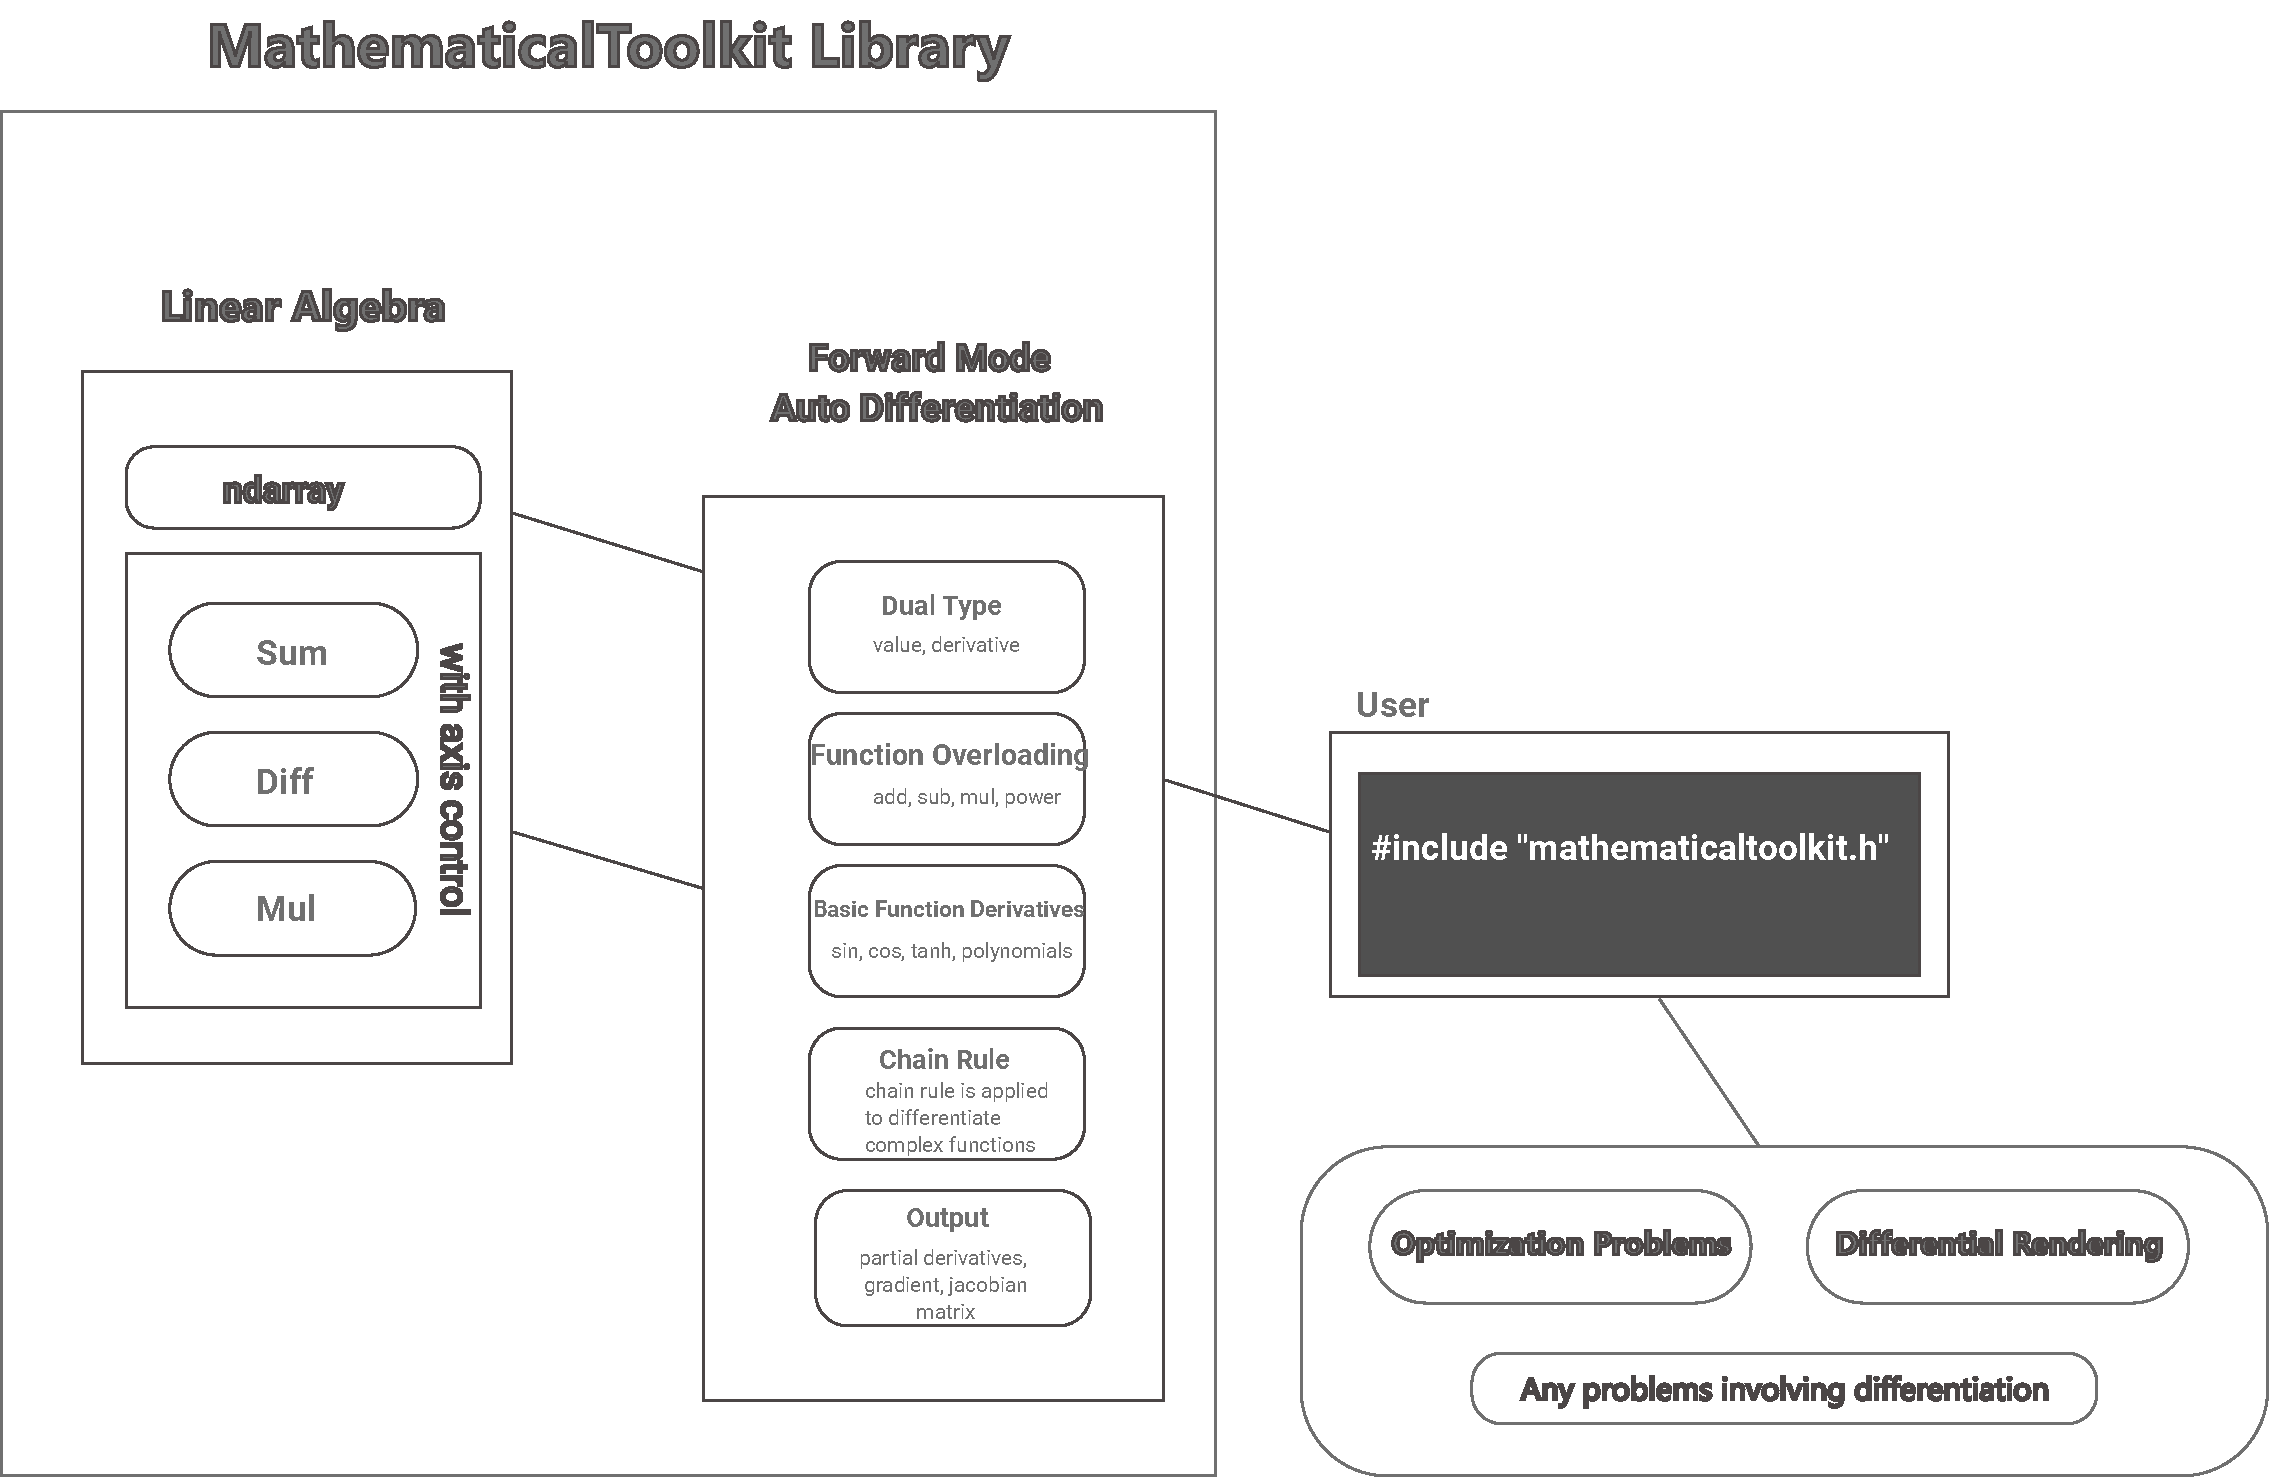
\includegraphics[width=1\linewidth,height = 12cm,scale=1.0]{Component-2-1.pdf}
	\centering
	\caption{Block Diagram for our System}
	\label{fig:BlockDiag}
\end{figure}
\end{center}

\newpage
\section{Methodology}
\begin{center}
\begin{figure}[htb]
	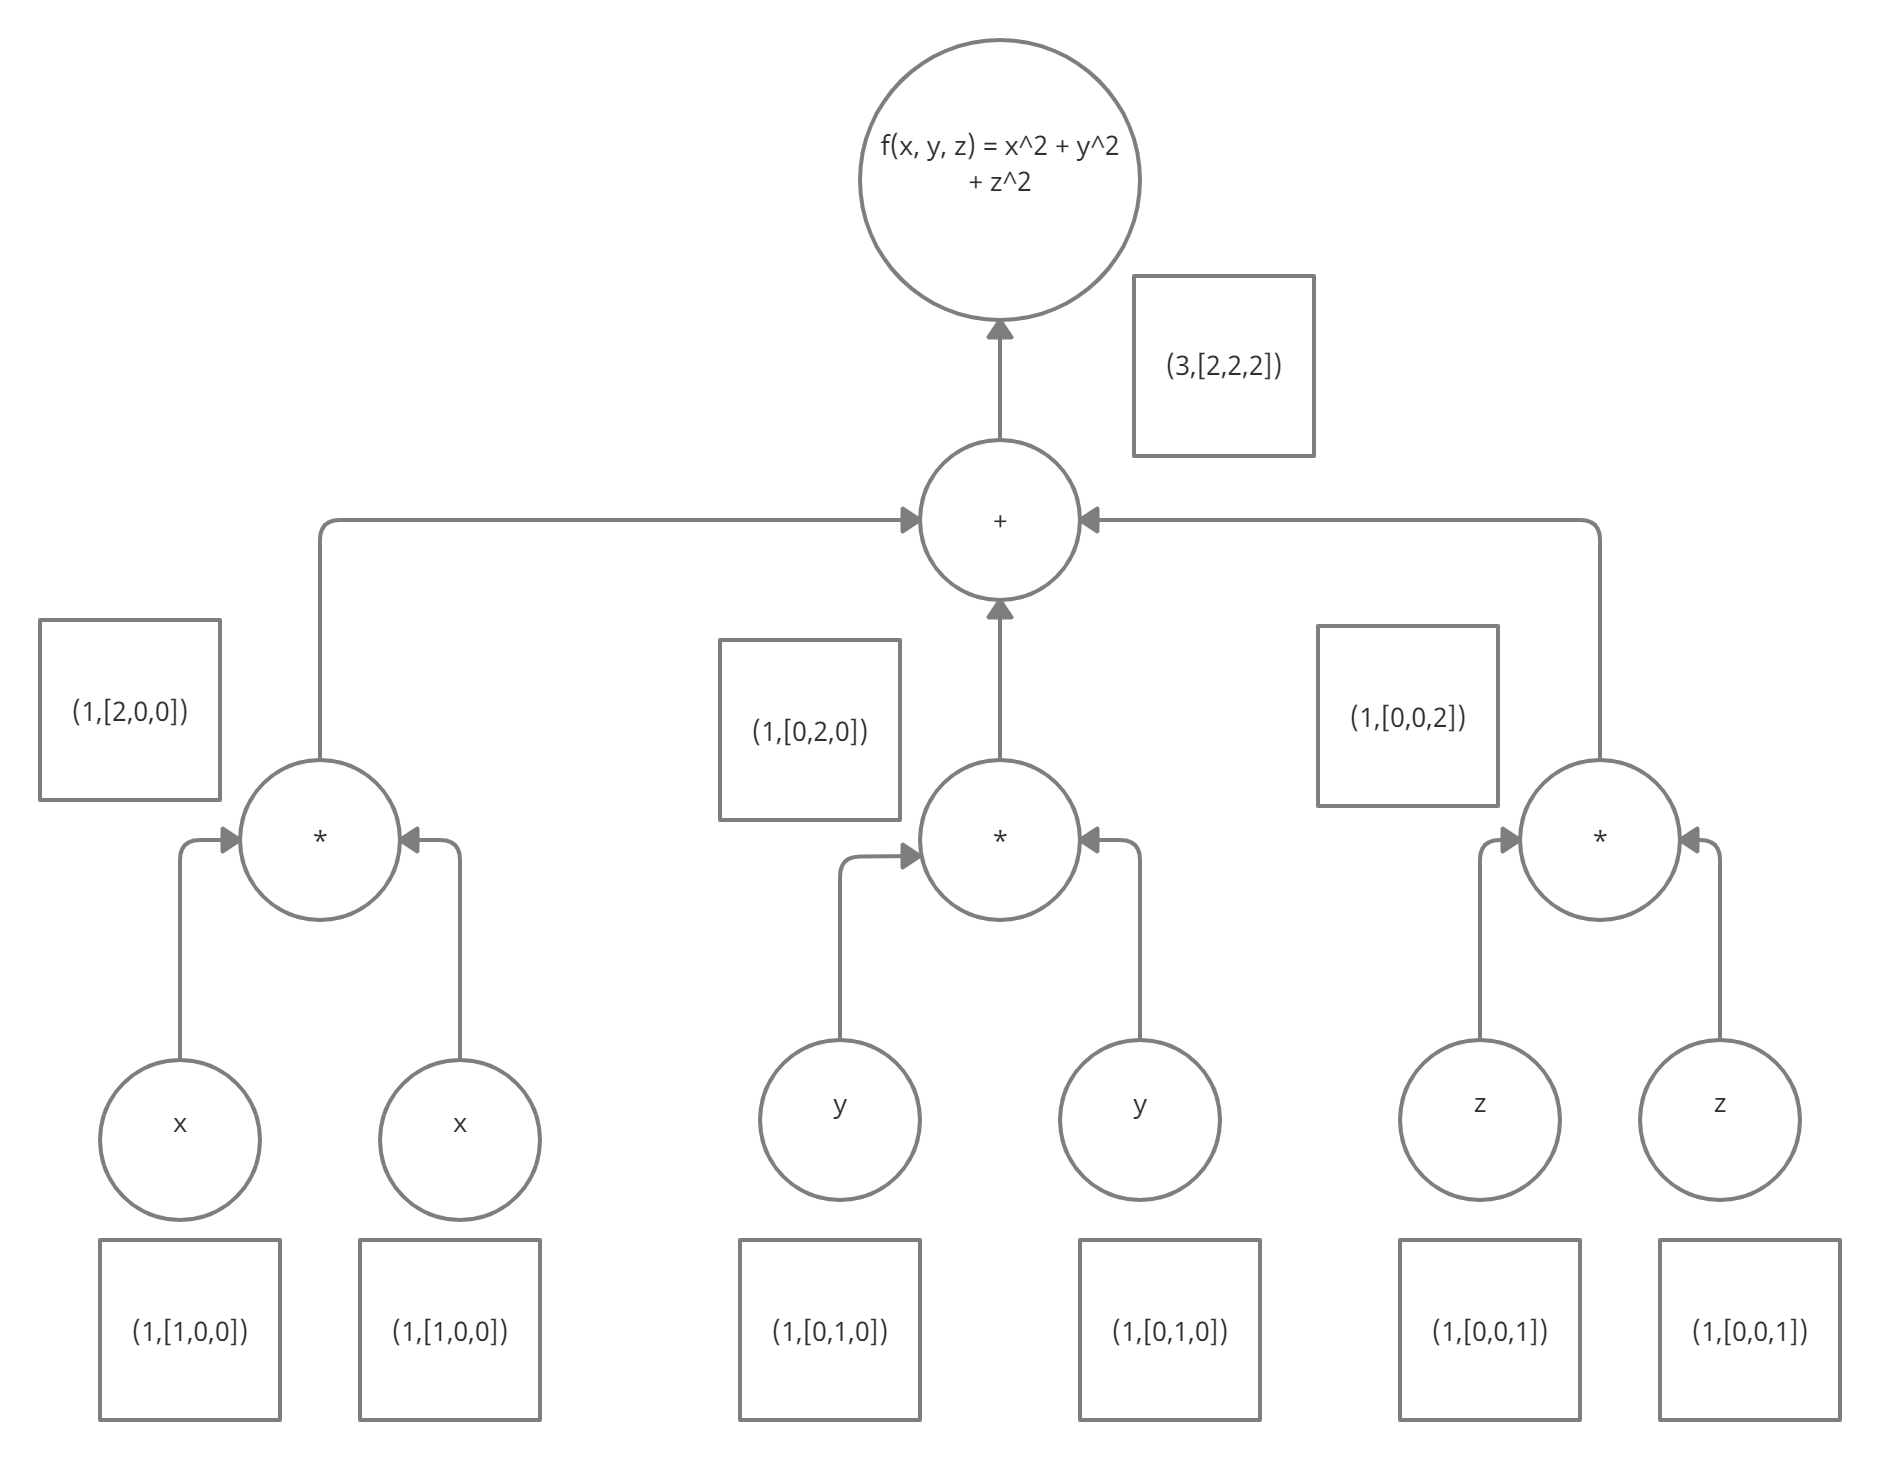
\includegraphics[width=0.8\linewidth, scale=0.6]{graph.jpg}
	\centering
	\caption{Forward Pass of the Primal and Gradient Values
			Over the Computational Graph}
	\label{fig:compgraph}
\end{figure}
\end{center}
The Graph in Figure~\ref{fig:compgraph} shows the computation 
of the gradient of the 3-variable square of the $L_{2}$ norm function 
in a single pass.
By creating a Multidimensional Dual class which has a primal 
value alongside a gradient vector, and then overloading the 
different arithmetic operators that we normally come across 
in everyday computations over this class, we can create a 
fully functioning \emph{gradient-computing} software.
We, could use the existing standard vector (std::vector) implementation
of the C++ standard library, however, since our project for
this semester is a very \textbf{\emph{Proof-Of-Concepts}}, we inted to 
try out our own vector class for this library.
\begin{lstlisting}[caption=How we could create our Dual Number class: ]
template <size_t N, typename T>
class NDual
{
	private: 	
		T primal;
		std::vector<T> grad(N);
	public:
		//relevant constructors, destructors, ...	
		//overloading the operators over the dual type 
};
\end{lstlisting}
The simple class template in the above listing can form the 
basis of our entire library.
We intend to learn and analyze object oriented best practices 
to come up with a memory safe and fairly optimized library.

\section{Project Scope}
Differentiation of functions, expressions written as computer programs
is extremely important. We have had ways of calclating the 
square root of something in computers forever. In C++, one could use
the $sqrt()$ function of the standard library. However, when it comes to 
differentiations, no such features are available. It becomes incredibly 
cumbersome for a programmer or any computer user to write their own 
code to differentiate a function and that's the issue we intend to solve
with MathematicalToolkit.


As data sets grow larger and larger, the fields like deep 
learning(see\cite{Goodfellow-et-al-2016}) require sophisticated 
Mathematical software for their usage. Though, we cannot promise 
our project in the Second Year of Engineering to match advanced 
implementations like Flux (see\cite{Fluxjl-2018},\cite{innes:2018}) and TensorFlow (see\cite{abadi2016tensorflow}),
we hope to get a grasp of most of these ideas under the object oriented 
paradigm which also happens to be the industry standard.



\section{Project Schedule}
The project is under development currently
\footnote{\label{MathematicalToolkit}https://github.com/yamisukehiro27/MathematicalToolkit}.
We intend to share our final project with the class come presentation 
day and it is supposed to be finished by the month of August.
The project should take about three and a half weeks for its completion.
As we work on our library, we intend to also create some examples
that can be helpful for users to see the capabilities of our library.


\newpage
\printbibliography
%\bibliographystyle{plain}
%\bibliography{bibilo}


\end{document}



%
% \documentclass[12pt]{article}
% \usepackage{dirtree}
% %\usepackage{cite}
% \usepackage[utf8]{inputenc}
% \usepackage{listings}
% \usepackage{pdfpages}
% \usepackage{fancyhdr}
% \usepackage{biblatex}
% \addbibresource{M335.bib}
% \usepackage{tocloft}
% %\renewcommand{\cftsecleader}{\cftdotfill{\cftdotsep}}
% %\renewcommand{\cftsecpagefont}{}% Remove \bfseries from section titles' page in ToC
% \usepackage{verbatim}
% \usepackage{amsmath}
% \usepackage[utf8]{inputenc}
% %\newcommand\logoPath{TU-logo.png}
% %\newcommand\logoFileName{TU-logo}
% %\newcommand\logoScaleFactor{0.7}
% \usepackage{graphicx}
% \usepackage{setspace}
% \usepackage{afterpage}
% \usepackage{tikz}
% \usetikzlibrary{shapes,arrows, positioning}
% \usepackage{abstract}
% \renewcommand{\abstractnamefont}{\normalfont\large\bfseries}
% \begin{document}
% \graphicspath{\logoPath}
% \renewcommand*\contentsname{Table Of Contents}
% \newcommand\myemptypage{
% 		\null
% 		\thispagestyle{empty}
% 		\addtocounter{page}{-1}
% 		\newpage
% }
% \lstdefinestyle{mystyle}{frame=tb,
% 						%language=C++,
% 						tabsize=3,
% 						numbersep=5pt}
% \lstset{style=mystyle}
% \begin{titlepage}
%   \begin{center}
%       \textbf{
%       	  \begin{huge}Project Proposal:\\ \end{huge}
%       	  \begin{huge}
%       	  GeoCold\\
% 			Ray Tracer (Differentiable?) in C++
% 			\end{huge}}\\
%     \vspace{0.5\baselineskip}
%     {\Large Authors:  Prakash Chaulagain, Nishar Arjyal, and Pramish Paudel}\\
%    	\Large{Roll Numbers: 076BCT045, 076BCT042, 076BCT047} \\
%    	\vspace{0.5\baselineskip}
%     \centering
%       Submitted to the Department of
%       Electronics and Computer Engineering
%       in Partial Fulfillment of the Requirements of the 3rd Year \textbf{Computer Graphics} Course  
%     at 	\\
%     {\Large Pulchowk Campus }\\
%     {\Large IOE, Tribhuwan University}\\
%     \vspace{0.3\baselineskip}
%     \today\\
%   \end{center}
%   \vspace{2\baselineskip}
%   {
%   \raggedright
% 		Accepted by: \dotfill
%
%   \raggedleft
%   \vspace{1\baselineskip}
%   Mr. Basanta Joshi\\
%   Assistant Professor at \\
%   The Department of Electronics and Computer Engineering\\
%   }
%   \vspace{2\baselineskip}	
% 	 Date of Submission: \today \\
%   	Expected Date of Completion: August, 2022 
% \end{titlepage}
% \myemptypage
% \begin{center}
% 	{\large \textbf{Mathematical Toolkit}}\\
% 	by
% 	{Prakash Chaulagain, Nishar Arjyal, and Pramish Paudel}\\
% 	\vspace{0.2\baselineskip}
% 	\begin{spacing}{0.8}
% 	{Submitted to the Department of Electronics and Computer Engineering \\
% 	on \today \\ in Partial Fulfillment of the Requirements for the 3rd Year 
% 	Computer Graphics Course in Computer Engineering}\\
% 	\end{spacing}
% \end{center}
% \begin{abstract}
% Derivatives and matrices seem to be ubiquitous in all of mathematical 
% optimization and machine learning nowadays. In such times, it becomes
% all the more important that the average computer programmer has access
% to a software package that is powerful yet simple to learn in order to 
% do fast gradient computations alongside a linear algebra package that-
% while-using feels native to the programming language of choice. The purpose
% of this project is to come up with one such mathematical package to 
% fulfil the requirements of academics for either soft-core academic work 
% or small-scale projects that require some form of mathematical optimization
% in C++. With MathematicalToolkit we aim to give the user a native C++ 
% experience in calculating derivatives of their functions.\\
% Several different methods exist for calculating the derivatives of 
% functions. Numerical and Symbolic are the first that come to mind. However, 
% when it comes to computer programming, the programming world seems to 
% have unanimously decided that the best method for a computer to differentiate
% functions is by using a set of techniques called Automatic Differentiation
% (see \cite{griewank} ).
% Automatic Differentiation (AD) is simply the most efficient family of 
% techniques for accurately calculating the derivatives of 
% functions. Several techniques exist in AD (see \cite{baydin2018automatic}), 
% however, the goal of this project is to implement only the Forward-Mode Automatic Differentiation
% using the operator overloading approach. This project also aims 
% to build a wrapper linear algebra sub-package for simple yet efficient 
% matrix and vector related computations.
%
% \end{abstract}
%
% \newpage
%
%
% \tableofcontents
% \newpage
%
% \begin{section}{Acknowledgement}
% 	Our project idea is the product of excellent supervision of all of our 
% 	instructors, most notably our lecturer Mr. Basanta Joshi. We could not 
% 	have been able to develop interest in computer graphics as a field of study 
% 	without the constant inspiration provided to us by all of our lecturers and 
% 	lab instructors and assistants. Some of the credit should also go to 
% 	the college administration for their efforts in the smooth functioning 
% 	of all of our classes and labs safely and securely despite the unprecedented 
% 	times of the pandemic. 
% \end{section}
%
% \newpage
%
% \newpage
% \pagestyle{fancy}
% \fancyhead[C]{MATHEMATICALTOOLKIT}
% \fancyhead[L]{}
% \renewcommand{\headrulewidth}{0pt}
% \renewcommand{\footrulewidth}{0pt}
% \section{Objectives}
% \begin{itemize}
% 	\item To bring Automatic Differentiation in a mathematical library
% 			that is suitable to use for academics.
% 	\item To analyze Object Oriented Programming design. 
% 	\item To get familiar with program optimization and safe memory-handling
% 	practices.
% \end{itemize}
% \section{Introduction}
% The most popularly used method for the computation of derivatives of 
% functions or mathematical expressions in computer program form when
% it comes to mathematical optimization problems or machine learning 
% is \emph{automatic differentiation}, also called 
% \emph{algorithmic differentiation} which is the major subject 
% matter of this project. 
%
% Conventionally, most of the algorithms of optimization have 
% relied heavily on computing derivatives and gradients of functions
% (see \cite{kochenderfer}\footnote{\label{kochenderfer}https://mitpress.mit.edu/books/algorithms-optimization}).
% Multiple implementations of automatic differentiation exist in 
% various programming languages such as in C++ (Carpenter et al., 2015 \cite{carpenter2015stan})
% as well as some higher level programming languages like Julia (see \cite{RevelsLubinPapamarkou2016})
% However, most of these implementations are built to be used specifically
% in machine learning and not for academic work. Furthermore, most 
% such implementations are the reverse mode automatic 
% differentiation which is more suitable in machine learning but 
% perhaps less suitable in mathematics as we normally use. We aim to 
% provide a very naive and incredibly hackable AD package that is 
% usable for the clueless as much as it is for the pros. 
%
%
% %\subsection{Finite Differencing:}
% %Before talking about our implementation of automatic differentiation
% %, we would like to express that MathematicalToolkit also aims to 
% %provide to the user the facility of numeric differencing.
% %The Taylor's expansion of a function $f(x)$ about a point $a$ $(x-a=h)$ as a funciton 
% %of $x$ is: 
% %$$
% %f(x) = \sum_{n=0}^{\infty}\cfrac{f^{(n)}(a)}{n!}(x-a)^{(n)}
% %$$
% %This gives us a forward difference of a function at $a$ using only the 
% %first order terms with small difference as:
% %\begin{equation}
% %f'(a) \approx \cfrac{f(a+h)-f(a)}{h} 
% %\end{equation}
% %In case of a function with multiple variables, our library intends the user 
% %the following facility:
% %
% %If $f(\textbf{x})$ is a function of multiple variables $\textbf{x}$ where
% %$\textbf{x}$ is of length n, the gradient of such a function is 
% %evaluated at point $\textbf{a}$ by calculating the directional 
% %derivatives in the concerned direction and storing the results in 
% %a vector in the stack.
% %Here, \textbf{a} has the same size as \textbf{x}.
% %\begin{equation}
% %	\nabla f(\textbf{a}) = \left[ \cfrac{\partial f(\textbf{a})}{\partial x_{i}}\right] for~i = 0:n-1
% %\end{equation}
%
% \subsection{Scalar Dual Numbers and Forward Mode AD}
% The \emph{scalar dual number} type implemented in our library is defined as: 
% \begin{equation}
% 	\boxed{
% 		f(x + y\epsilon) = f(x) + yf'(x)\epsilon + \mathcal{O}(\epsilon^{2})
% }
% 	\label{scalardualdefine}
% \end{equation}
% The definition of the scalar dual number in equation~\ref{scalardualdefine}
% contains a primal/value part '$x$' and a derivative part '$y$'.
% Following eqn.~\ref{scalardualdefine}, we obtain 
% the derivative of any function through eqn.~\ref{dualdiff}
% \begin{equation}
% 	\boxed{
% 	f'(x) = \cfrac{f(x+y\epsilon) - f(x)}{y\epsilon}
% }
% 	\label{dualdiff}
% \end{equation}
% By defining some dual number arithmetic through operator overloading 
% such as: 
% \begin{equation}
% 	\boxed{
% 	(x_{1}+y_{1}\epsilon) + (x_{2}+y_{2}\epsilon) = (x_{1}+x_{2}) + (y_{1}+y_{2})\epsilon
% }
% 	\label{dualadd}
% \end{equation}
% We can achieve this easily by overloading the '+' operator over 
% our custom scalar '\emph{Dual}' type. 
% \\
%
% The eqn.\ref{dualmult} is the definition of the product of two dual types.
% \begin{equation}
% 	\boxed{
% 	(x_{1}+y_{1}\epsilon) \times (x_{2}+y_{2}\epsilon) = (x_{1}x_{2}) + (x_{1}y_{2}+x_{2}y_{1})\epsilon
% }
% 	\label{dualmult}
% \end{equation}
% So, basically we are defining the basic derivative formulae on the 
% dual type, and for chained functions, we define a set of chain rules. 
% In this way, we can obtain the derivative of all scalar functions that depend
% on only one variable.
% \\
% The $\epsilon$ in all of these formulae is called the $machine-epsilon$
% defined as: $\epsilon^{2} = 0$ in the computer.
% The epsilon is defined as such: 
% 1.0 + $\epsilon$ == 1.0 returns a true in the computer program.
% So, basically, when we add or subtract a number from or to an $\epsilon$
% we have done literally no computation. Further, all higher powers of 
% $\epsilon$ are zero.
% \subsection{Multidimensional Dual Numbers and Vector Forward Mode AD}
% The scalar type mentioned above works suitably for scalar one-variable 
% functions; however, better approach can be taken in the case of 
% multivariate functions.
% \\
% Let's analyze how we can differentiate a function of two variables 
% using our scalar dual numbers.
% The $L_{2}$ norm of a vector $\overrightarrow{x}$ of length $n$ is defined to 
% be (the indices are chosen to be the same as those used in programming 
% normally).
%
% \begin{equation}
% 	\boxed{
% 	||\overrightarrow{x}|| = \left(\sum_{i=0}^{i=n-1}x_{i}^{2}\right)^{\cfrac{1}{2}}
% }
% 	\label{l2norm}
% \end{equation}
% Let us try finding the gradient of the square of this functions when the input 
% has two elements.
% \begin{equation}
% 	\boxed{
% f(x_{0},x_{1}) = x_{0}^{2} + x_{1}^{2}
% }
% \end{equation}
% First, the partial derivative with respect to $x_{0}$ is found 
% by noticing that the derivative of $x_{0}$ w.r.t. $x_{0}$ itself is 
% 1 and the  derivative of $x_{1}$ w.r.t. $x_{0}$ is 0. \\
% So basically, we are passing the dual number into the function which 
% returns the value alongside the derivative as a dual number.
% \begin{align}
% 	f(x_{0}+\epsilon, x_{1}) &= (x_{0}+\epsilon)^{2} + x_{1}^{2}  \\
% 	f(x_{0}+\epsilon, x_{1}) &= x_{0}^{2} + 2x_{0}\epsilon + \epsilon^{2} + x_{1}^{2} \\
% 	f(x_{0}+\epsilon, x_{1}) &= (x_{0}^{2}+x_{1}^{2})+ 2x_{0}\epsilon  
% \end{align}
% Notice from the second equation above to the third, we used the definition 
% that $\epsilon^{2}$ is 0 and so are all higher powers of $\epsilon$
% \\
% So, the value of $f(x_{0}, x_{1})$ at $(x_{0},x_{1})$ is 
% $x_{0}^{2}+x_{1}^{2}$ while the partial derivative of $f(x_{0},x_{1})$ w.r.t.
% $x_{0}$ is $2x_{0}$
% This method becomes clearly very rigorous if the input has a large size when 
% it comes to making gradient computations.
% We only had to calculate the derivative w.r.t. one input here. 
% For the gradient, we would need to set the derivative part
% of $x_{0}$ equal to zero just like we set the derivative part of $x_{1}$ to
% zero in the above equations and set the derivative part of $x_{1}$ to 1.
% In both the cases, we would get a dual number with the same primal/value
% parts but the derivative parts would separately be the partial derivative of 
% the function with respect to $x_{0}$ and $x_{1}$.
% So, we can reduce redundancy by wrapping our input and the dual number 
% into a vector. We introduce the multidimensioanl dual number type in our package.
% The multidimensional dual number type implemented in MathematicalToolkit 
% is very much so based on the paper \cite{RevelsLubinPapamarkou2016} and is 
% defined as such for a scalar function:
% \begin{equation}
% 	f(x+\sum_{i = 1}^{k}y_{i}\epsilon_{i}) = f(x) + f'(x)\sum_{i=1}^{k}y_{i}\epsilon_{i}
% \end{equation}
% The product of all $\epsilon_{i}\epsilon_{j}$ is zero by definition.
% For the case in which the function depends upon multiple variables: 
% \begin{equation}
% 	\overrightarrow{x} = \begin{bmatrix}x_{1}\\ \vdots \\ x_{i} \\ \vdots \\ x_{k} \end{bmatrix} \rightarrow \overrightarrow{x_{\epsilon}}
% 	= \begin{bmatrix}x_{1}+\epsilon_{1}+0\sum_{n=2}^{k}\epsilon_{n}
% 	\\
% 	\vdots \\
% 	x_{i}+\epsilon_{i}+0\sum_{n\neq i}\epsilon_{n}
% 	\\
% 	\vdots \\
% 	x_{k}+\epsilon_{k} + 0\sum_{n=1}^{k-1}\epsilon_{n}
%
% 	\end{bmatrix} = \begin{bmatrix}
% 	x_{1}+\epsilon_{1} \\ \vdots \\ x_{i}+\epsilon_{i}\\ \vdots 
% 	\\ x_{k}+\epsilon_{k}
% 					\end{bmatrix}
% 					\rightarrow f(\overrightarrow{x}_{\epsilon}) = f(\overrightarrow{x})
% 					+ \sum_{i=1}^{k}\cfrac{\partial{f(\overrightarrow{x})}}{\partial{x_{i}}}\epsilon_{i}
% 	\label{multidimdual}
% \end{equation}
%
% Now, we can calculate the gradient of $f(x_{0},x_{1})$ from before as such:
% First, for the first component of the gradient:
% $$
% f\left(\begin{bmatrix}x_{0} + \epsilon_{0}\\x_{1}+\epsilon_{1}\end{bmatrix}\right)
% = x_{0}^{2}+2x_{0}\epsilon_{0}+x_{1}^{2}+2x_{0}\epsilon_{1}
% =(x_{0}^{2}+x_{1}^{2})+\epsilon_{0}(2x_{0})+\epsilon_{1}(2x_{1})
% $$
% So, in one single pass, we have calculated the value of $\nabla{f(\overrightarrow{x})}$
% to be : $\left<2x_{0}, 2x_{1}\right>$.
%
% \section{Existing Systems}
% Several implementations of the  Forward and Vector Forward Mode AD 
% or even Reverse Mode AD exist already. Perhaps the most popular such 
% library is TensorFlow(see \cite{abadi2016tensorflow})\footnote{\label{tenserflow}https://github.com/tensorflow/tensorflow} 
% (some people may not have been acquaintained with the fact that
% TensorFlow is an AD software but it is).
% TensorFlow applies a \emph{trace-based} implementation of the reverse-mode
% AD. A popular such tool implemented using operator overloading in C++ 
% is ADOL-C (see\cite{adol:c})\footnote{\label{adol-c} https://github.com/coin-or/ADOL-C}.
% A popular high-level implementaton of the vector forward-mode AD is in a 
% Julia package called ForwardDiff.jl (see \cite{RevelsLubinPapamarkou2016})
% \footnote{\label{ForwardDiff}https://github.com/JuliaDiff/ForwardDiff.jl}.
% The Stan Math Library (see \cite{carpenter2015stan}) is a C++ implementation 
% of reverse mode automatic differentiation (\cite{griewank}).
% Fast AD (see\cite{yang2021fastad}) is a C++ AD library based on Expresion 
% Templates.
%
% \section{Proposed System}
% \subsection{Description}
% The user should be able to use our package after downloading and then
% doing a '\emph{build}' of the package on their system. The library should 
% be \emph{callable} in one's program by doing something as simple as:
% \\
% \#\textbf{include} $<$MathematicalToolkit$>$
%
% The user should be able to write the following code and have their gradients
% computed:
% \begin{lstlisting}[caption=What Using MathematicalToolkit Would Feel Like]
% #include <iostream>
% #include <MathematicalToolkit> //including the library header file
% grad::NDual f(grad::NDual x,grad::NDual y)
% {
% 	return x*x + y*y;   //f(x,y) = sq(x) + sq(y)
% }
% int main()
% {	
% 	double eps1[] = {1,0}
% 	double eps2[] = {0,1};
% 	grad::NDual x(1.0,eps1);
% 	grad::NDual y(1.0,eps2); //will give the gradient of x*x+y*y at
% 	f(x,y).grad::gradient(); //x = 1.0, y = 1.0							
% }
% \end{lstlisting}
%
% A program as simple as this should give to the user the gradient of the 
% function. Obviously, the final thing that we intend to serve would
% be capable to do more than just this; however, this is only a simple glimpse 
% of what our library is supposed to bring. We intend our library to 
% work comfortably with numerous most common mathematical functions 
% and data types.
% \\
% The library is supposed to be type generic as much as possible and 
% one of the goals is to write the source code of the library in a way that
% is possible and easy for everyone to read and get a grasp of what is 
% going on under the hood.
% Our package is also supposed to provide to the user a simple 
% linear algebra wrapper library that makes it possible to solve
% systems of linear equations, as well as constructing Vandermonde matrices
% which find their usage in \emph{Polynomial Interpolation}, among many other
% features one would normally expect of a linear algebra library.
% \\
% Our program should be made available at GitHub as an Open Source Project.
% The directory structure followed by our project should be relatively 
% simple and follow the common directory tree structure of most of the C++ 
% libraries.
% \
% \newpage
% The package is suppposed to have the following directory structure:
% \\
% \dirtree{%
% 	.1 MathematicalToolkit.
% 	.2 docs.
% 	.2 include.
% 	.2 src.  
% 	.2 test.  
% } 
% Thus, following the industry standard of creating C++ libraries.\\
% In the final product, we intend to show examples of what are the possibilities
% that one can unlock using our library. We intend to show some 
% visualization of \emph{Polynomial Curve Fitting} as well as some \emph{Optimization
% Algorithms} at work using MathematicalToolkit.
%
% \subsection{System Block Diagram}
% The following is a block diagram of our system:
% \begin{center}
% \begin{figure}[htb]	
% 	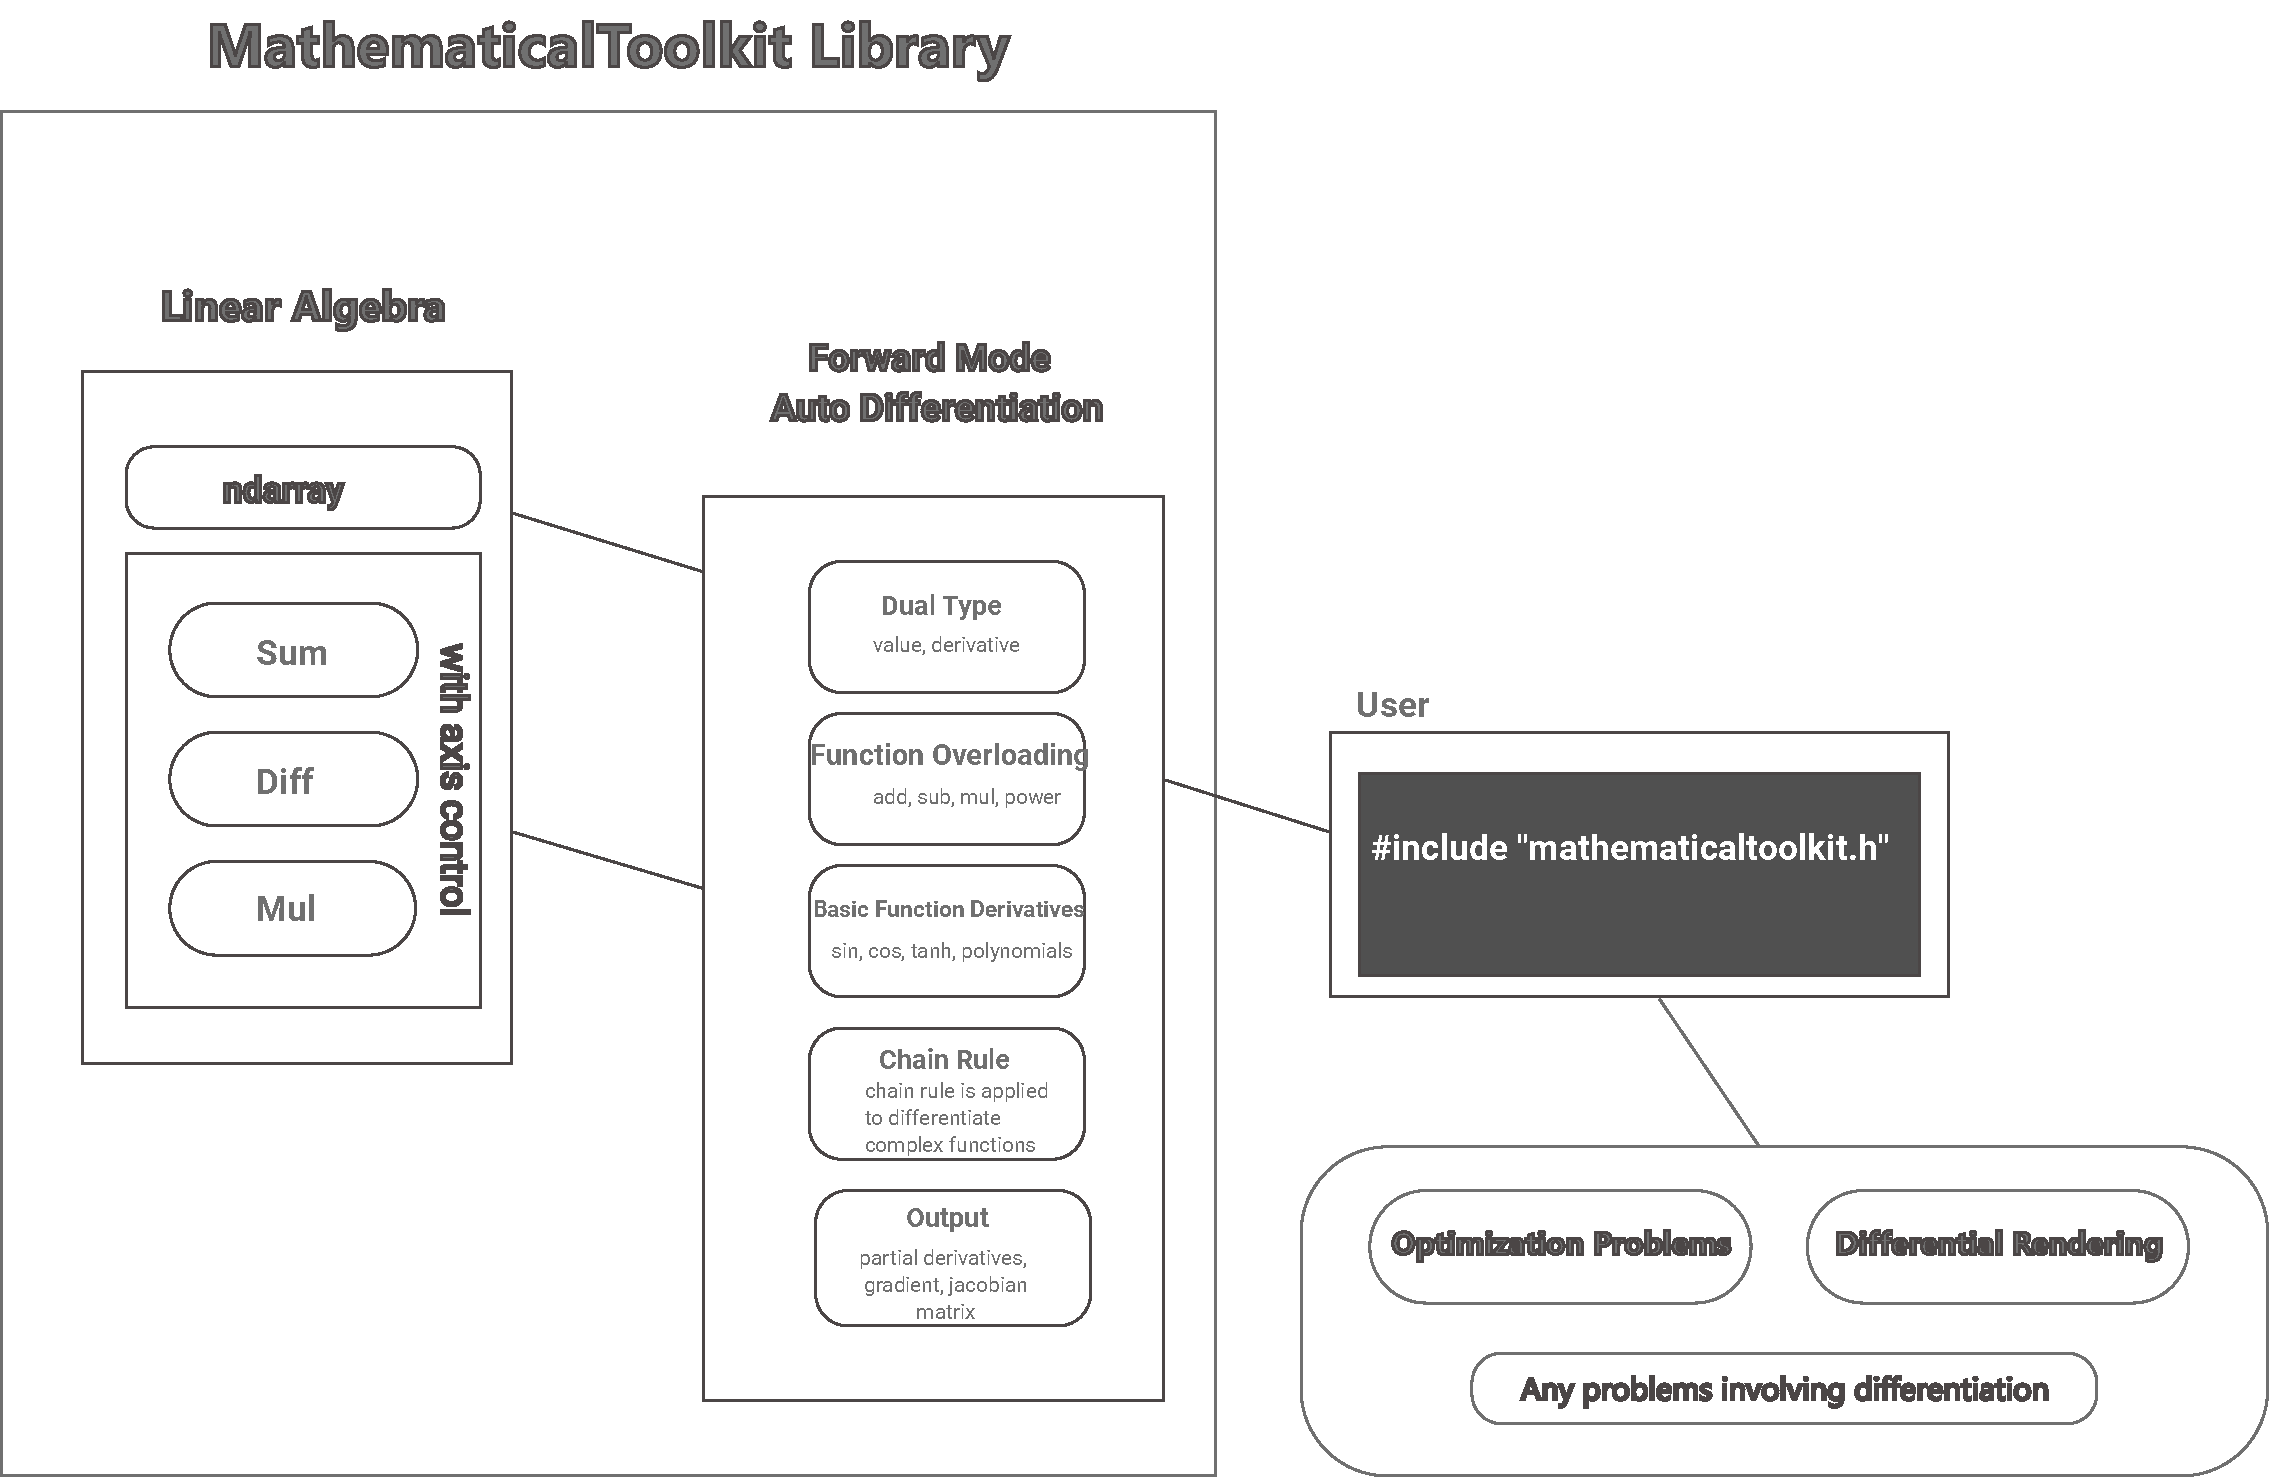
\includegraphics[width=1\linewidth,height = 12cm,scale=1.0]{Component-2-1.pdf}
% 	\centering
% 	\caption{Block Diagram for our System}
% 	\label{fig:BlockDiag}
% \end{figure}
% \end{center}
%
% \newpage
% \section{Methodology}
% \begin{center}
% \begin{figure}[htb]
% 	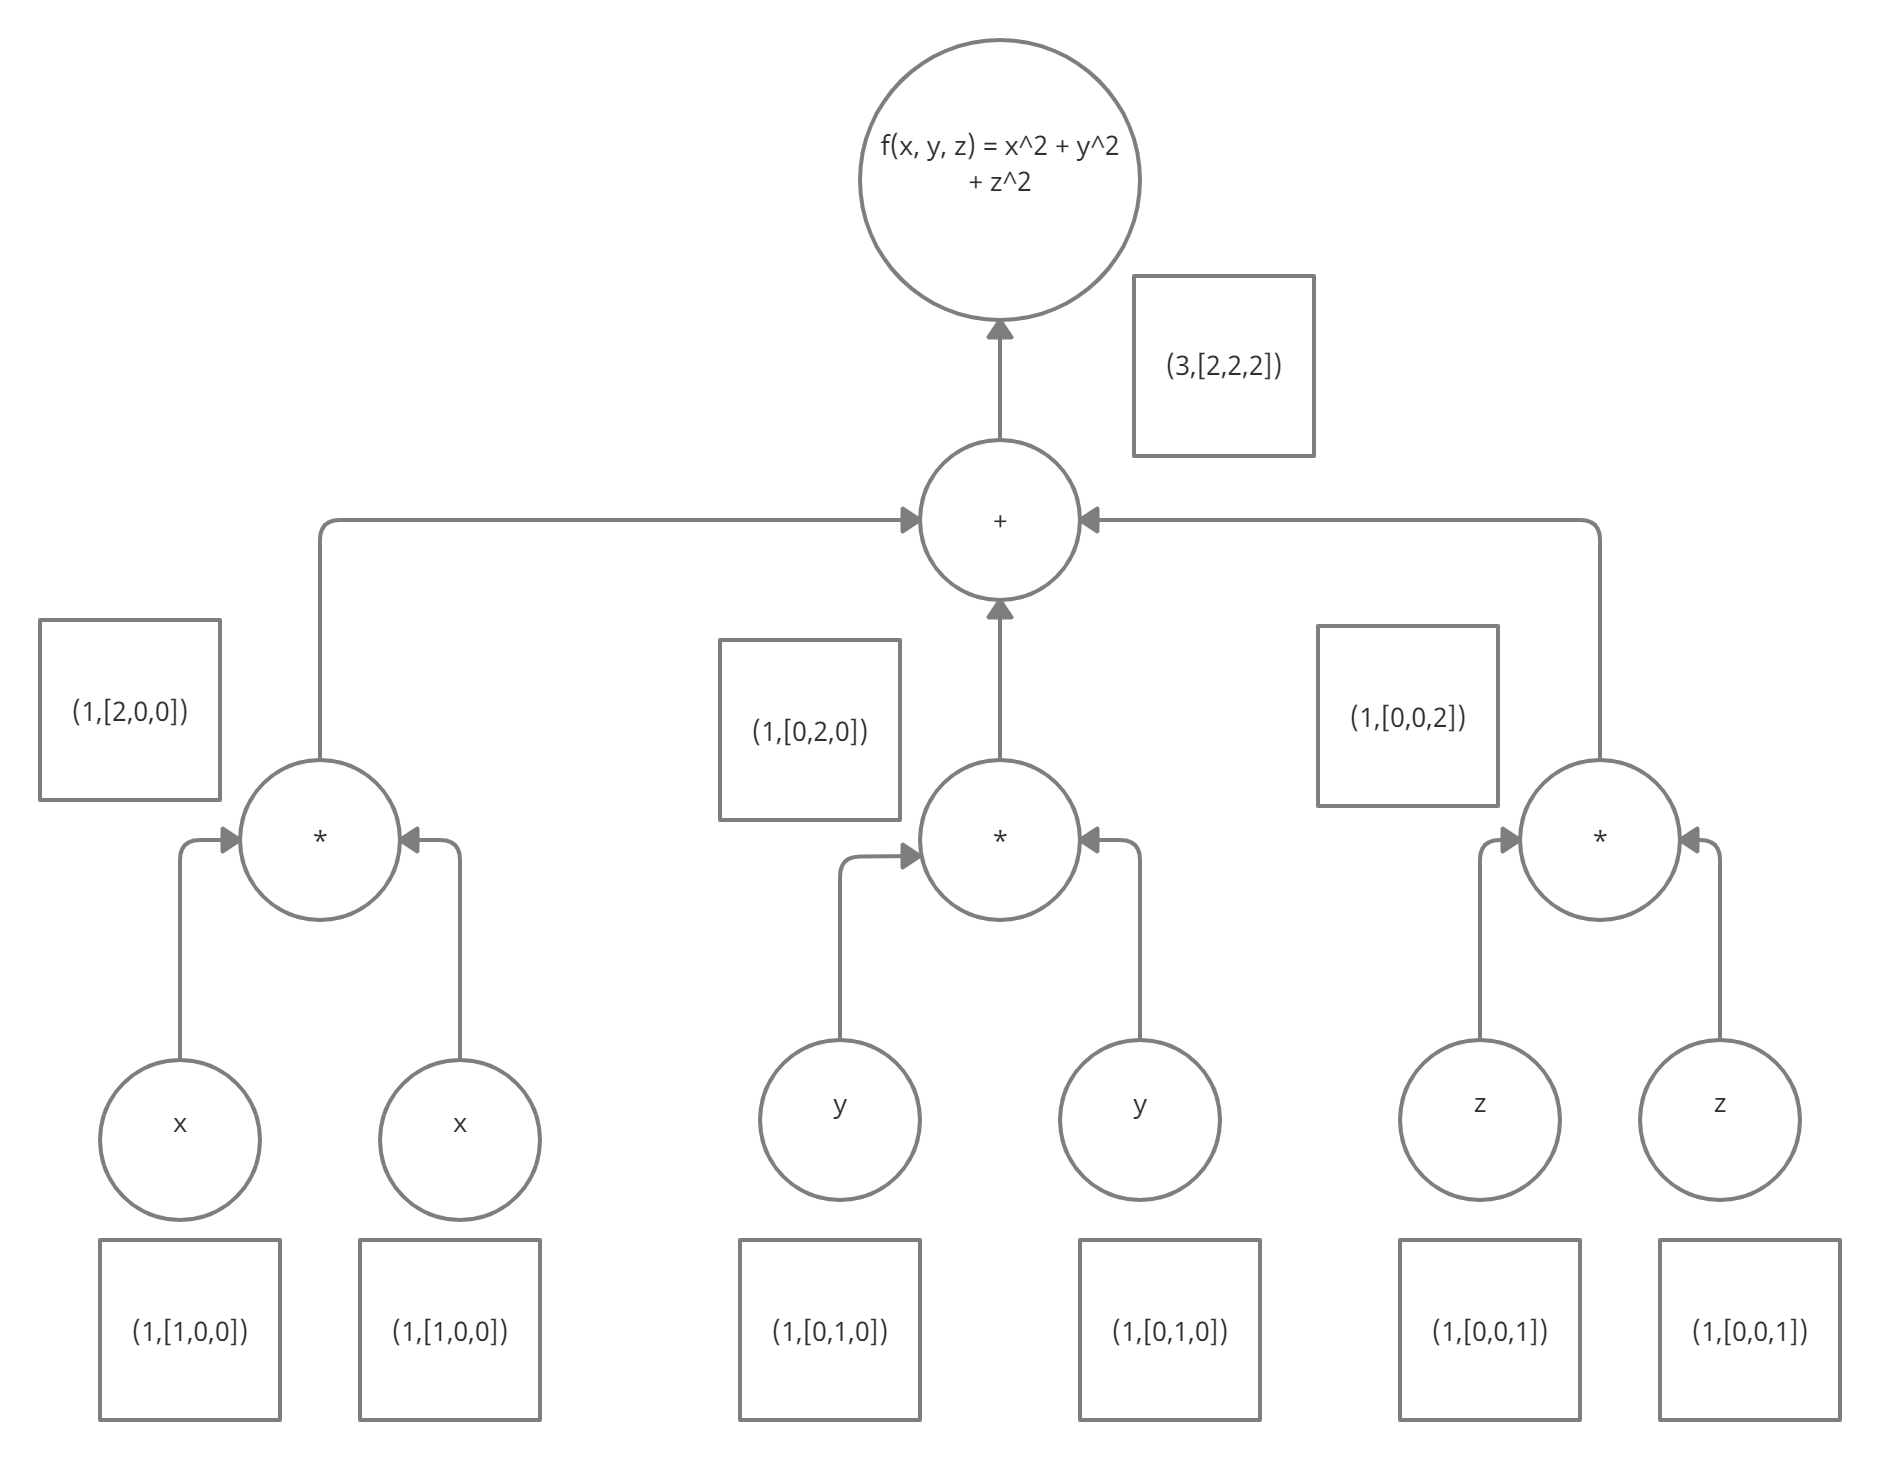
\includegraphics[width=0.8\linewidth, scale=0.6]{graph.jpg}
% 	\centering
% 	\caption{Forward Pass of the Primal and Gradient Values
% 			Over the Computational Graph}
% 	\label{fig:compgraph}
% \end{figure}
% \end{center}
% The Graph in Figure~\ref{fig:compgraph} shows the computation 
% of the gradient of the 3-variable square of the $L_{2}$ norm function 
% in a single pass.
% By creating a Multidimensional Dual class which has a primal 
% value alongside a gradient vector, and then overloading the 
% different arithmetic operators that we normally come across 
% in everyday computations over this class, we can create a 
% fully functioning \emph{gradient-computing} software.
% We, could use the existing standard vector (std::vector) implementation
% of the C++ standard library, however, since our project for
% this semester is a very \textbf{\emph{Proof-Of-Concepts}}, we inted to 
% try out our own vector class for this library.
% \begin{lstlisting}[caption=How we could create our Dual Number class: ]
% template <size_t N, typename T>
% class NDual
% {
% 	private: 	
% 		T primal;
% 		std::vector<T> grad(N);
% 	public:
% 		//relevant constructors, destructors, ...	
% 		//overloading the operators over the dual type 
% };
% \end{lstlisting}
% The simple class template in the above listing can form the 
% basis of our entire library.
% We intend to learn and analyze object oriented best practices 
% to come up with a memory safe and fairly optimized library.
%
% \section{Project Scope}
% Differentiation of functions, expressions written as computer programs
% is extremely important. We have had ways of calclating the 
% square root of something in computers forever. In C++, one could use
% the $sqrt()$ function of the standard library. However, when it comes to 
% differentiations, no such features are available. It becomes incredibly 
% cumbersome for a programmer or any computer user to write their own 
% code to differentiate a function and that's the issue we intend to solve
% with MathematicalToolkit.
%
%
% As data sets grow larger and larger, the fields like deep 
% learning(see\cite{Goodfellow-et-al-2016}) require sophisticated 
% Mathematical software for their usage. Though, we cannot promise 
% our project in the Second Year of Engineering to match advanced 
% implementations like Flux (see\cite{Fluxjl-2018},\cite{innes:2018}) and TensorFlow (see\cite{abadi2016tensorflow}),
% we hope to get a grasp of most of these ideas under the object oriented 
% paradigm which also happens to be the industry standard.
%
%
%
% \section{Project Schedule}
% The project is under development currently
% \footnote{\label{MathematicalToolkit}https://github.com/yamisukehiro27/MathematicalToolkit}.
% We intend to share our final project with the class come presentation 
% day and it is supposed to be finished by the month of August.
% The project should take about three and a half weeks for its completion.
% As we work on our library, we intend to also create some examples
% that can be helpful for users to see the capabilities of our library.
%
%
% \newpage
% \printbibliography
% %\bibliographystyle{plain}
% %\bibliography{bibilo}
%
%
% \end{document}
%
%
